Before we discuss how BitShares achieves price \emph{stability} we first need to
define what properties make a currency \emph{stable}.

In the U.S., for instance, the Federal Reserve (FED) has a mandate of
\emph{stable prices} and it is almost universally accepted that this is a good
mandate. The same holds true for the Euro with its stability being
\emph{controlled} by the European Central Bank (ECB). Mostly every
country/nation or federation applies a similar concept to gain control over
prices via monetary policies like quantitative easing and interest rates for
commercial banks that borrow money the central bank.

As a very basic example, imagine a central bank managed to keep prices stable
through their monetary policy with 0\% price inflation over 20 years. Now lets
assume that during this same 20 years the advances in robotics and automation
resulted in a 3x increase in efficiency and thus there are now 3x as much food,
cars, phones, houses, etc. For the sake of this example we will assume the
population is the same and everyone has the same amount of money in the bank.
You would normally expect that everything would be 1/3 the price and that
everyone would be able to afford 3x their prior life style. But because of the
central bank's intervention they have managed to also increase the money supply
by 3x. The newly created money is then borrowed to the commercial banks which
borrow it again to the people at a profit.

Since this monetary inflation is a sustained increase in the general level of
prices, it is equivalent to a decline in purchasing power of money.  Hence, a
dollar buys less and less over time. As a result, we see the dollar losing 99\%
of its \emph{purchasing power} since the FED was founded in 1913~(see
\cref{fig:monetarybase}). 

\begin{figure}[!htp]
 \centering
 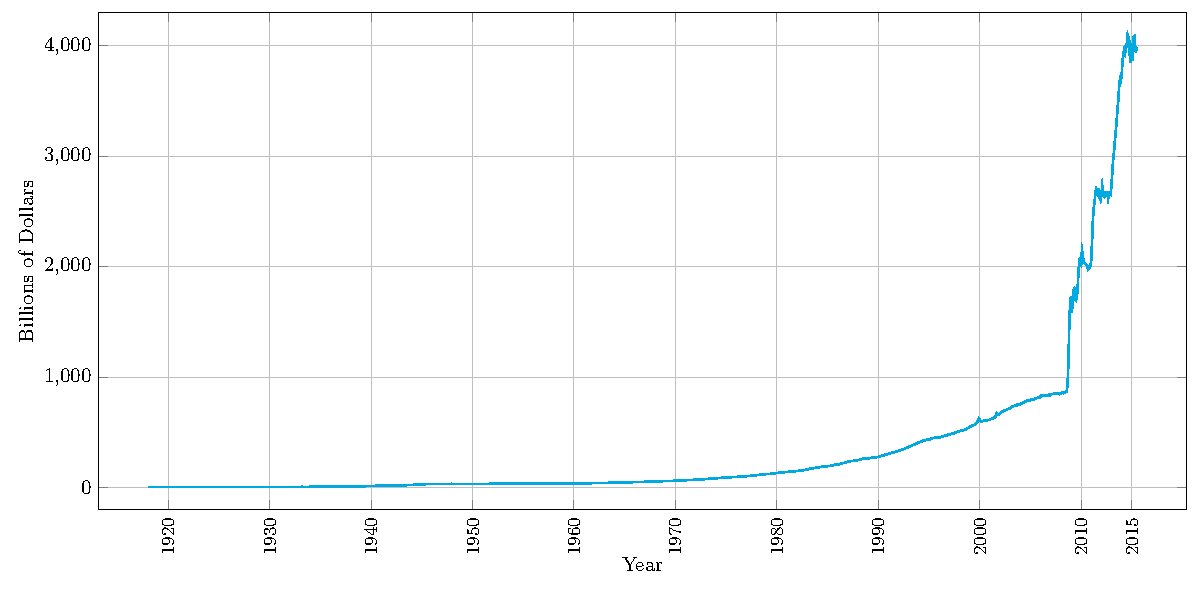
\includegraphics[width=\linewidth]{figures/monetary-base}
 \caption{St. Louis Adjusted Monetary Base~\cite{ambsl}}
 \label{fig:monetarybase}
\end{figure}

Of course, the goal of this paper is not to propose a replacement of central
banks or their monetary policies, but to clarify the terminology in particular
with regards to ``stable'' cryptocurrencies. Unfortunately, some people in the
cryptocurrency space are attempting to provide an alternative currency that can
achieve the same mandate as the central banks and leave the profits in the
hands of only few institutional entities. For this reason, we do not want to
bring this same mandate to crypto currencies but instead aim for a
decentralized solution.

From the example above, we notice that the goals should not be \emph{price
stability} nor should we target a \emph{stable value} or \emph{purchasing
power} (at least not yet). 
%
What we want to achieve instead is 
\begin{itemize}
 \item a \emph{predictable} price with \emph{reduced volatility}
 \item a somewhat reliable ability to \emph{predict the future value} of a token, and
 \item a unit of account that doesn't have any meaningful capital gains or
       losses for tax purposes.
\end{itemize}

Hence, for us, price ``stability'' means price \emph{predictability} within
some tolerance level. In the case of the U.S. dollar, a willingness to accept a
yearly loss in purchasing power via monetary policies, demonstrates that
predictability is more important than stability~\cite{bm:stable:impossible}.



% Since price stability at its heart is the same as \emph{price fixing}, this is
% a well known economic fallacy that crypto-currencies should avoid.
%
% The goal of the FED price stability mandate is to mask the systematic theft of
% all increases in the production efficiency of the economy. 
%
% and distribute it in secret. The end result is that some people get a 1000x
% increase in life style while everyone else stands still.
%
% We can conclude from this example that the mandate for price stability is
% mostly a goal meant to mislead the general public and mask theft from the lower
% and middle classes on a massive scale even at 0\% price inflation. 
